

\tikzset{every picture/.style={line width=0.75pt}} %set default line width to 0.75pt        

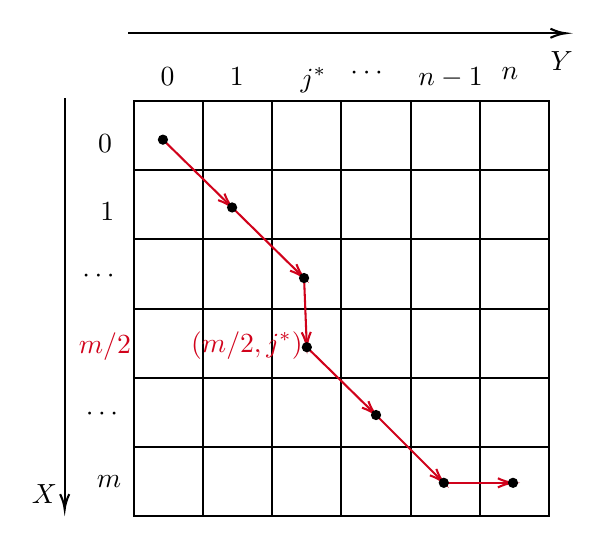
\begin{tikzpicture}[x=0.5pt,y=0.5pt,yscale=-1,xscale=1]
%uncomment if require: \path (0,424); %set diagram left start at 0, and has height of 424

%Shape: Grid [id:dp24675112085229023] 
\draw  [draw opacity=0] (87,90) -- (387,90) -- (387,390) -- (87,390) -- cycle ; \draw   (137,90) -- (137,390)(187,90) -- (187,390)(237,90) -- (237,390)(287,90) -- (287,390)(337,90) -- (337,390) ; \draw   (87,140) -- (387,140)(87,190) -- (387,190)(87,240) -- (387,240)(87,290) -- (387,290)(87,340) -- (387,340) ; \draw   (87,90) -- (387,90) -- (387,390) -- (87,390) -- cycle ;
%Straight Lines [id:da19565394910393163] 
\draw    (37,88) -- (37,383) ;
\draw [shift={(37,385)}, rotate = 270] [color={rgb, 255:red, 0; green, 0; blue, 0 }  ][line width=0.75]    (10.93,-3.29) .. controls (6.95,-1.4) and (3.31,-0.3) .. (0,0) .. controls (3.31,0.3) and (6.95,1.4) .. (10.93,3.29)   ;
%Straight Lines [id:da01702598838428071] 
\draw    (83,41) -- (397,41) ;
\draw [shift={(399,41)}, rotate = 180] [color={rgb, 255:red, 0; green, 0; blue, 0 }  ][line width=0.75]    (10.93,-3.29) .. controls (6.95,-1.4) and (3.31,-0.3) .. (0,0) .. controls (3.31,0.3) and (6.95,1.4) .. (10.93,3.29)   ;
%Straight Lines [id:da2874309790229619] 
\draw [color={rgb, 255:red, 208; green, 2; blue, 27 }  ,draw opacity=1 ]   (108,117.9) -- (156.57,165.5) ;
\draw [shift={(158,166.9)}, rotate = 224.42] [color={rgb, 255:red, 208; green, 2; blue, 27 }  ,draw opacity=1 ][line width=0.75]    (10.93,-3.29) .. controls (6.95,-1.4) and (3.31,-0.3) .. (0,0) .. controls (3.31,0.3) and (6.95,1.4) .. (10.93,3.29)   ;
%Straight Lines [id:da632617045829971] 
\draw [color={rgb, 255:red, 208; green, 2; blue, 27 }  ,draw opacity=1 ]   (262,316.9) -- (309.59,364.48) ;
\draw [shift={(311,365.9)}, rotate = 225] [color={rgb, 255:red, 208; green, 2; blue, 27 }  ,draw opacity=1 ][line width=0.75]    (10.93,-3.29) .. controls (6.95,-1.4) and (3.31,-0.3) .. (0,0) .. controls (3.31,0.3) and (6.95,1.4) .. (10.93,3.29)   ;
%Straight Lines [id:da4311447007524547] 
\draw [color={rgb, 255:red, 208; green, 2; blue, 27 }  ,draw opacity=1 ]   (311,365.9) -- (359,365.9) ;
\draw [shift={(361,365.9)}, rotate = 180] [color={rgb, 255:red, 208; green, 2; blue, 27 }  ,draw opacity=1 ][line width=0.75]    (10.93,-3.29) .. controls (6.95,-1.4) and (3.31,-0.3) .. (0,0) .. controls (3.31,0.3) and (6.95,1.4) .. (10.93,3.29)   ;
%Straight Lines [id:da42492070365720014] 
\draw [color={rgb, 255:red, 208; green, 2; blue, 27 }  ,draw opacity=1 ]   (158,166.9) -- (208.57,216.5) ;
\draw [shift={(210,217.9)}, rotate = 224.44] [color={rgb, 255:red, 208; green, 2; blue, 27 }  ,draw opacity=1 ][line width=0.75]    (10.93,-3.29) .. controls (6.95,-1.4) and (3.31,-0.3) .. (0,0) .. controls (3.31,0.3) and (6.95,1.4) .. (10.93,3.29)   ;
%Straight Lines [id:da782029434490156] 
\draw [color={rgb, 255:red, 208; green, 2; blue, 27 }  ,draw opacity=1 ]   (210,217.9) -- (211.92,265.9) ;
\draw [shift={(212,267.9)}, rotate = 267.71] [color={rgb, 255:red, 208; green, 2; blue, 27 }  ,draw opacity=1 ][line width=0.75]    (10.93,-3.29) .. controls (6.95,-1.4) and (3.31,-0.3) .. (0,0) .. controls (3.31,0.3) and (6.95,1.4) .. (10.93,3.29)   ;
%Straight Lines [id:da04914804346774482] 
\draw [color={rgb, 255:red, 208; green, 2; blue, 27 }  ,draw opacity=1 ]   (212,267.9) -- (260.57,315.5) ;
\draw [shift={(262,316.9)}, rotate = 224.42] [color={rgb, 255:red, 208; green, 2; blue, 27 }  ,draw opacity=1 ][line width=0.75]    (10.93,-3.29) .. controls (6.95,-1.4) and (3.31,-0.3) .. (0,0) .. controls (3.31,0.3) and (6.95,1.4) .. (10.93,3.29)   ;
%Shape: Circle [id:dp6219757716700797] 
\draw  [fill={rgb, 255:red, 0; green, 0; blue, 0 }  ,fill opacity=1 ] (105.1,117.9) .. controls (105.1,116.3) and (106.4,115) .. (108,115) .. controls (109.6,115) and (110.9,116.3) .. (110.9,117.9) .. controls (110.9,119.5) and (109.6,120.79) .. (108,120.79) .. controls (106.4,120.79) and (105.1,119.5) .. (105.1,117.9) -- cycle ;
%Shape: Circle [id:dp14254311997747549] 
\draw  [fill={rgb, 255:red, 0; green, 0; blue, 0 }  ,fill opacity=1 ] (155.1,166.9) .. controls (155.1,165.3) and (156.4,164) .. (158,164) .. controls (159.6,164) and (160.9,165.3) .. (160.9,166.9) .. controls (160.9,168.5) and (159.6,169.79) .. (158,169.79) .. controls (156.4,169.79) and (155.1,168.5) .. (155.1,166.9) -- cycle ;
%Shape: Circle [id:dp08471894355443155] 
\draw  [fill={rgb, 255:red, 0; green, 0; blue, 0 }  ,fill opacity=1 ] (207.1,217.9) .. controls (207.1,216.3) and (208.4,215) .. (210,215) .. controls (211.6,215) and (212.9,216.3) .. (212.9,217.9) .. controls (212.9,219.5) and (211.6,220.79) .. (210,220.79) .. controls (208.4,220.79) and (207.1,219.5) .. (207.1,217.9) -- cycle ;
%Shape: Circle [id:dp15806530128538276] 
\draw  [fill={rgb, 255:red, 0; green, 0; blue, 0 }  ,fill opacity=1 ] (209.1,267.9) .. controls (209.1,266.3) and (210.4,265) .. (212,265) .. controls (213.6,265) and (214.9,266.3) .. (214.9,267.9) .. controls (214.9,269.5) and (213.6,270.79) .. (212,270.79) .. controls (210.4,270.79) and (209.1,269.5) .. (209.1,267.9) -- cycle ;
%Shape: Circle [id:dp03429229121700372] 
\draw  [fill={rgb, 255:red, 0; green, 0; blue, 0 }  ,fill opacity=1 ] (259.1,316.9) .. controls (259.1,315.3) and (260.4,314) .. (262,314) .. controls (263.6,314) and (264.9,315.3) .. (264.9,316.9) .. controls (264.9,318.5) and (263.6,319.79) .. (262,319.79) .. controls (260.4,319.79) and (259.1,318.5) .. (259.1,316.9) -- cycle ;
%Shape: Circle [id:dp43136430210698984] 
\draw  [fill={rgb, 255:red, 0; green, 0; blue, 0 }  ,fill opacity=1 ] (308.1,365.9) .. controls (308.1,364.3) and (309.4,363) .. (311,363) .. controls (312.6,363) and (313.9,364.3) .. (313.9,365.9) .. controls (313.9,367.5) and (312.6,368.79) .. (311,368.79) .. controls (309.4,368.79) and (308.1,367.5) .. (308.1,365.9) -- cycle ;
%Shape: Circle [id:dp4334570092838286] 
\draw  [fill={rgb, 255:red, 0; green, 0; blue, 0 }  ,fill opacity=1 ] (358.1,365.9) .. controls (358.1,364.3) and (359.4,363) .. (361,363) .. controls (362.6,363) and (363.9,364.3) .. (363.9,365.9) .. controls (363.9,367.5) and (362.6,368.79) .. (361,368.79) .. controls (359.4,368.79) and (358.1,367.5) .. (358.1,365.9) -- cycle ;

% Text Node
\draw (68,103) node [anchor=north west][inner sep=0.75pt]   [align=left] {$ $};
% Text Node
\draw (60.5,161.38) node [anchor=north west][inner sep=0.75pt]   [align=left] {$\displaystyle 1$};
% Text Node
\draw (11,365) node [anchor=north west][inner sep=0.75pt]   [align=left] {$\displaystyle X$};
% Text Node
\draw (386,52) node [anchor=north west][inner sep=0.75pt]   [align=left] {$\displaystyle Y$};
% Text Node
\draw (104,63.44) node [anchor=north west][inner sep=0.75pt]   [align=left] {$\displaystyle 0$};
% Text Node
\draw (290.4,63.44) node [anchor=north west][inner sep=0.75pt]   [align=left] {$\displaystyle n-1$};
% Text Node
\draw (59,112) node [anchor=north west][inner sep=0.75pt]   [align=left] {$\displaystyle 0$};
% Text Node
\draw (47.5,209.76) node [anchor=north west][inner sep=0.75pt]   [align=left] {$\displaystyle \cdots $};
% Text Node
\draw (58,358.5) node [anchor=north west][inner sep=0.75pt]   [align=left] {$\displaystyle m$};
% Text Node
\draw (154.1,63.44) node [anchor=north west][inner sep=0.75pt]   [align=left] {$\displaystyle 1$};
% Text Node
\draw (205.2,63.44) node [anchor=north west][inner sep=0.75pt]   [align=left] {$\displaystyle j^{*}$};
% Text Node
\draw (350.5,63.44) node [anchor=north west][inner sep=0.75pt]   [align=left] {$\displaystyle n$};
% Text Node
\draw (241.3,63.44) node [anchor=north west][inner sep=0.75pt]   [align=left] {$\displaystyle \cdots $};
% Text Node
\draw (126.2,254.44) node [anchor=north west][inner sep=0.75pt]   [align=left] {$\displaystyle \textcolor[rgb]{0.82,0.01,0.11}{\left( m/2,j^{*}\right)}$};
% Text Node
\draw (50,309.5) node [anchor=north west][inner sep=0.75pt]   [align=left] {$\displaystyle \cdots $};
% Text Node
\draw (45,255.5) node [anchor=north west][inner sep=0.75pt]   [align=left] {$\displaystyle \textcolor[rgb]{0.82,0.01,0.11}{m/2}$};


\end{tikzpicture}

